\documentclass[12pt,a4paper]{article}
\usepackage[utf8]{inputenc}
\usepackage[T1]{fontenc}
\usepackage{amsmath,amssymb,amsfonts}
\usepackage{geometry}
\usepackage{listings}
\usepackage{xcolor}
\usepackage{hyperref}
\usepackage{booktabs}
\usepackage{array}
\usepackage{tikz}
\usetikzlibrary{arrows.meta,shapes,positioning,calc,fit,backgrounds}

\geometry{margin=2.5cm}
\lstset{
  basicstyle=\ttfamily\footnotesize,
  keywordstyle=\color{blue!80}\bfseries,
  commentstyle=\color{gray}\itshape,
  stringstyle=\color{red!70},
  breaklines=true,
  frame=single,
  backgroundcolor=\color{gray!5},
  numbers=left,
  numberstyle=\tiny\color{gray},
  captionpos=b
}

\title{\textbf{Report 4: Commander Module}\\[0.4em]
\large \textbf{Part~I:} Complete Original System --- Every Function\\
\textbf{Part~II:} Every Soaring-Mode Modification and Its Impact\\[0.5em]
\normalsize PX4 Autosoaring Implementation --- Defence Technical Report}
\author{Radhouene --- Fixed-Wing Autosoaring Project}
\date{April 2026}

\begin{document}
\maketitle
\tableofcontents
\newpage

%=============================================================================
\section*{List of Symbols and Acronyms}
\addcontentsline{toc}{section}{List of Symbols and Acronyms}
%=============================================================================

\subsection*{Abbreviations}
\begin{center}\begin{tabular}{ll}\toprule
Symbol & Meaning \\\midrule
\texttt{uORB} & Micro Object Request Broker --- PX4's publish/subscribe IPC bus \\
\texttt{MAVLink} & Micro Air Vehicle Link --- binary telemetry/command protocol \\
\texttt{DDS} & Data Distribution Service --- middleware used by XRCE-DDS for ROS2 \\
CLI & Command-Line Interface \\
SITL & Software-In-The-Loop simulation \\
HIL & Hardware-In-The-Loop simulation \\
RTL & Return-To-Launch \\
GCS & Ground Control Station (e.g.\ QGroundControl) \\
VTOL & Vertical Take-Off and Landing \\
LED & Light-Emitting Diode (status indicator) \\
\bottomrule\end{tabular}\end{center}

\subsection*{Key uORB Topics Published / Subscribed by Commander}
\begin{center}\begin{tabular}{lll}\toprule
Topic & Direction & Content \\\midrule
\texttt{vehicle\_status} & Published & Navigation state, arming state, failsafe flags \\
\texttt{vehicle\_control\_mode} & Published & Boolean control-mode flags (altitude, position, etc.) \\
\texttt{actuator\_armed} & Published & Armed, prearmed, lockdown, force\_failsafe \\
\texttt{failure\_detector\_status} & Published & Failure detector roll/pitch/alt/motor flags \\
\texttt{vehicle\_command} & Subscribed & Incoming MAVLink-format commands \\
\texttt{vehicle\_command\_ack} & Published & Command acknowledgement result codes \\
\texttt{action\_request} & Subscribed & Arm/disarm/mode-switch requests from RC/joystick \\
\texttt{parameter\_update} & Subscribed & Signals parameter changes \\
\texttt{battery\_status} & Subscribed & Battery SOC/voltage for failsafe thresholds \\
\texttt{manual\_control\_input} & Subscribed & Pilot stick inputs \\
\texttt{mission\_result} & Subscribed & Mission finished/valid flags \\
\texttt{vehicle\_land\_detected} & Subscribed & Landed / in-air state \\
\texttt{power\_button\_state} & Subscribed & Physical power button events \\
\texttt{datalink\_status} & Subscribed & Telemetry link health \\
\texttt{offboard\_control\_mode} & Subscribed & Offboard mode setpoint validity \\
\bottomrule\end{tabular}\end{center}

\subsection*{Navigation State Constants (nav\_state field of vehicle\_status)}
\begin{center}\begin{tabular}{ll}\toprule
Constant & Flight mode \\\midrule
\texttt{NAVIGATION\_STATE\_MANUAL} & Manual (no autopilot) \\
\texttt{NAVIGATION\_STATE\_ALTCTL} & Altitude control \\
\texttt{NAVIGATION\_STATE\_POSCTL} & Position control \\
\texttt{NAVIGATION\_STATE\_AUTO\_MISSION} & Follow uploaded mission \\
\texttt{NAVIGATION\_STATE\_AUTO\_LOITER} & Circle a fixed point \\
\texttt{NAVIGATION\_STATE\_AUTO\_RTL} & Return to launch \\
\texttt{NAVIGATION\_STATE\_AUTO\_TAKEOFF} & Automatic takeoff \\
\texttt{NAVIGATION\_STATE\_AUTO\_LAND} & Automatic landing \\
\texttt{NAVIGATION\_STATE\_AUTO\_PRECLAND} & Precision landing \\
\texttt{NAVIGATION\_STATE\_ACRO} & Acrobatic / rate control \\
\texttt{NAVIGATION\_STATE\_STAB} & Stabilised (roll/pitch damped) \\
\texttt{NAVIGATION\_STATE\_OFFBOARD} & External position/velocity setpoints \\
\texttt{NAVIGATION\_STATE\_TERMINATION} & Kill switch / termination \\
\texttt{NAVIGATION\_STATE\_ORBIT} & GCS-commanded orbit \\
\bottomrule\end{tabular}\end{center}

\subsection*{MAVLink Command IDs used in Commander}
\begin{center}\begin{tabular}{ll}\toprule
Constant & Purpose \\\midrule
\texttt{VEHICLE\_CMD\_DO\_SET\_MODE} (176) & Switch flight mode \\
\texttt{VEHICLE\_CMD\_COMPONENT\_ARM\_DISARM} (400) & Arm or disarm motors \\
\texttt{VEHICLE\_CMD\_DO\_REPOSITION} (192) & Move loiter centre \\
\texttt{VEHICLE\_CMD\_PREFLIGHT\_CALIBRATION} (241) & Sensor calibration \\
\texttt{VEHICLE\_CMD\_RUN\_PREARM\_CHECKS} (401) & Run safety checks \\
\texttt{VEHICLE\_CMD\_PREFLIGHT\_REBOOT\_SHUTDOWN} (246) & Reboot / shutdown FMU \\
\texttt{VEHICLE\_CMD\_NAV\_TAKEOFF} (22) & Auto takeoff \\
\texttt{VEHICLE\_CMD\_NAV\_LAND} (21) & Auto land \\
\texttt{VEHICLE\_CMD\_DO\_FLIGHTTERMINATION} (185) & Lockdown / kill \\
\texttt{VEHICLE\_CMD\_DO\_VTOL\_TRANSITION} (3000) & MC$\leftrightarrow$FW transition \\
\texttt{VEHICLE\_CMD\_CUSTOM\_0} (31010) & User-defined; soaring mode here \\
\texttt{VEHICLE\_CMD\_FIXED\_MAG\_CAL\_YAW} (42006) & Fast magnetometer calibration \\
\bottomrule\end{tabular}\end{center}

\newpage
%=============================================================================
\part{Original Commander System}
%=============================================================================

%=============================================================================
\section{Module Purpose and Architecture}
%=============================================================================

\texttt{Commander} is the \emph{system state manager} and \emph{safety arbiter} of PX4.
It is the single authoritative source of the vehicle's \textbf{arming state} and
\textbf{navigation state}. Every other module reads these from the
\texttt{vehicle\_status} uORB topic; none of them switch states themselves.

Commander has no direct link to sensors or actuators. Its data flow is:

%--- Complete Commander Input / Output flow diagram ----------------------------
\begin{figure}[h!]
\centering
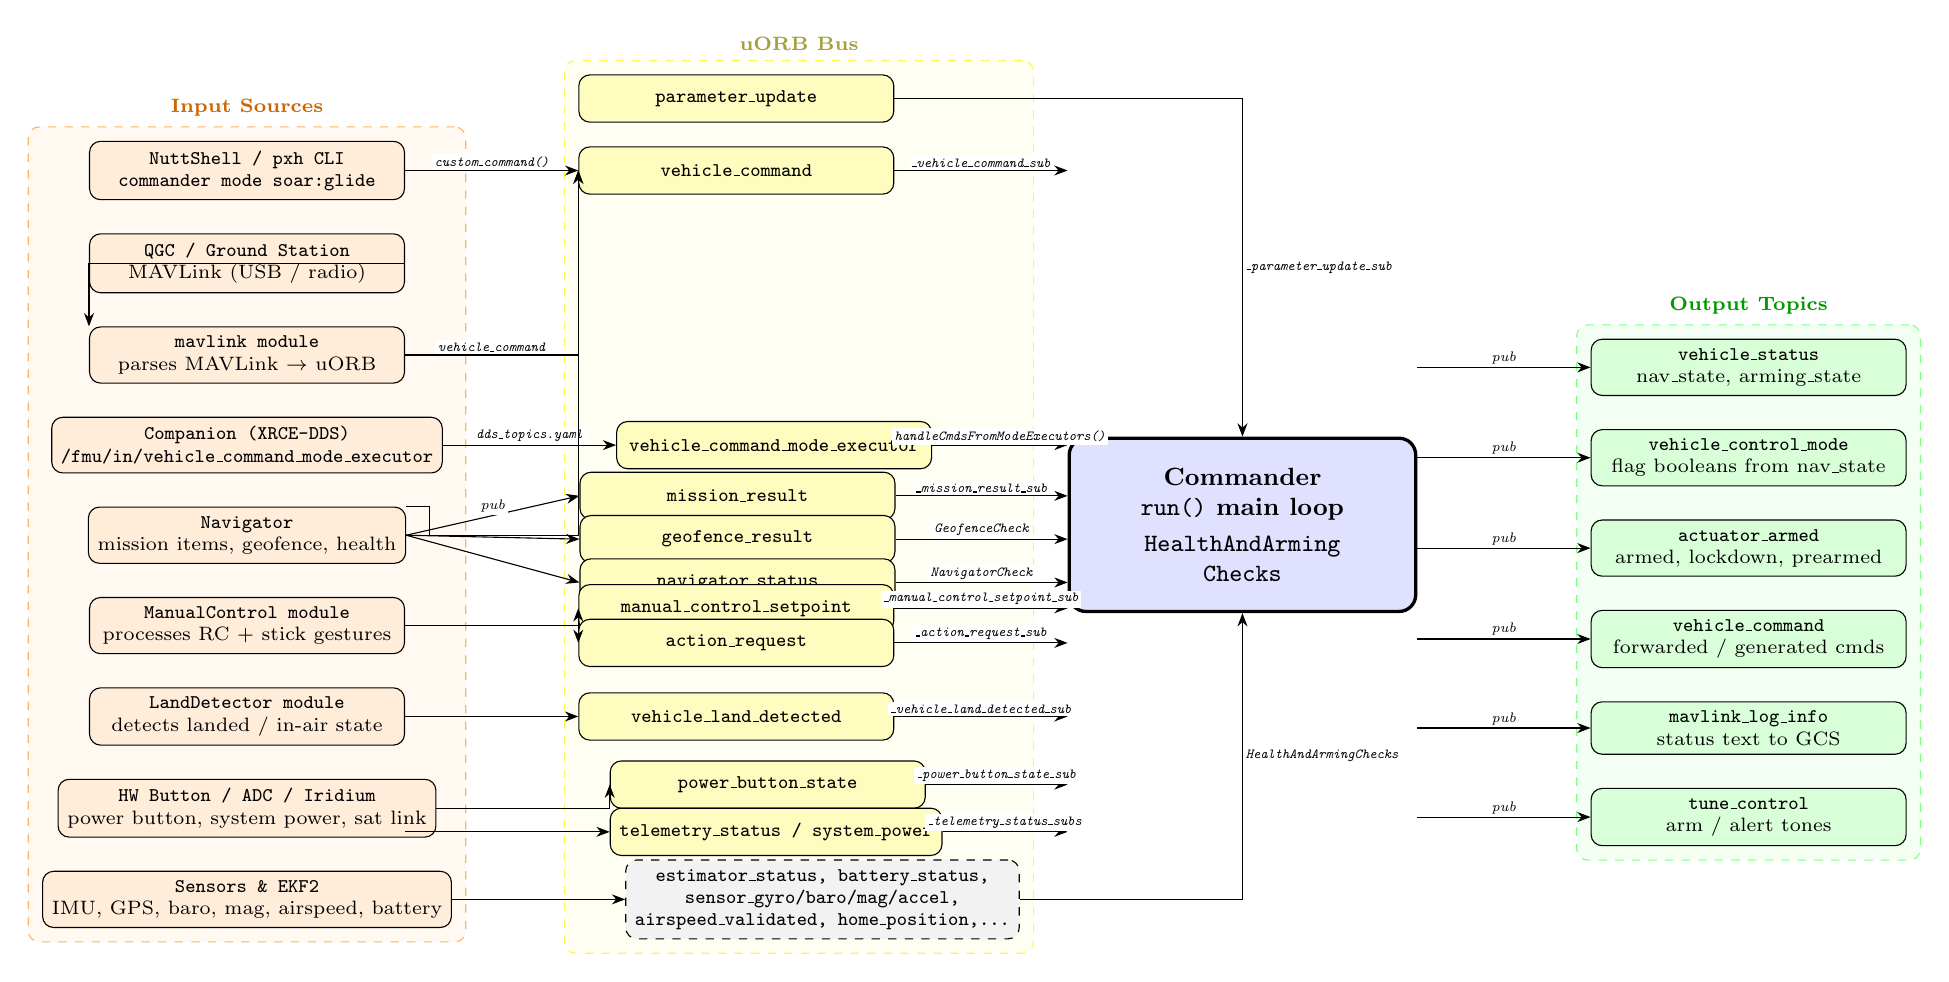
\begin{tikzpicture}[
  >=Stealth,
  src/.style   ={draw, rounded corners=4pt, fill=orange!15,
                 minimum width=4.0cm, minimum height=0.65cm,
                 align=center, font=\scriptsize\ttfamily},
  bus/.style   ={draw, rounded corners=4pt, fill=yellow!25,
                 minimum width=4.0cm, minimum height=0.60cm,
                 align=center, font=\scriptsize\ttfamily},
  core/.style  ={draw, very thick, rounded corners=6pt, fill=blue!12,
                 minimum width=4.4cm, minimum height=2.2cm,
                 align=center, font=\small\bfseries},
  outbox/.style={draw, rounded corners=4pt, fill=green!15,
                 minimum width=4.0cm, minimum height=0.60cm,
                 align=center, font=\scriptsize\ttfamily},
  sensbox/.style={draw, dashed, rounded corners=4pt, fill=gray!10,
                 minimum width=4.0cm, minimum height=0.60cm,
                 align=center, font=\scriptsize\ttfamily},
  arrlbl/.style={font=\tiny\itshape, midway, fill=white, inner sep=1pt},
  node distance = 0.42cm and 2.0cm
]

% ===== LEFT COLUMN: INPUT SOURCES ============================================
\node[src] (cli)
  {NuttShell / pxh CLI\\{\normalfont\texttt{commander mode soar:glide}}};

\node[src, below=of cli] (qgc)
  {QGC / Ground Station\\{\normalfont MAVLink (USB / radio)}};

\node[src, below=of qgc] (mav)
  {mavlink module\\{\normalfont parses MAVLink $\to$ uORB}};

\node[src, below=of mav] (cpn)
  {Companion (XRCE-DDS)\\{\normalfont \texttt{/fmu/in/vehicle\_command\_mode\_executor}}};

\node[src, below=of cpn] (nav)
  {Navigator\\{\normalfont mission items, geofence, health}};

\node[src, below=of nav] (mc)
  {ManualControl module\\{\normalfont processes RC + stick gestures}};

\node[src, below=of mc] (lnd)
  {LandDetector module\\{\normalfont detects landed / in-air state}};

\node[src, below=of lnd] (btn)
  {HW Button / ADC / Iridium\\{\normalfont power button, system power, sat link}};

\node[src, below=of btn] (ekf)
  {Sensors \& EKF2\\{\normalfont IMU, GPS, baro, mag, airspeed, battery}};

% ===== CENTRE-LEFT COLUMN: uORB TOPICS =======================================
\node[bus, right=2.2cm of cli]   (vcmd)
  {\texttt{vehicle\_command}};

\node[bus, right=2.2cm of cpn]   (vcme)
  {\texttt{vehicle\_command\_mode\_executor}};

\node[bus, right=2.2cm of nav, yshift= 0.50cm] (mres)
  {\texttt{mission\_result}};

\node[bus, right=2.2cm of nav, yshift=-0.05cm] (gfr)
  {\texttt{geofence\_result}};

\node[bus, right=2.2cm of nav, yshift=-0.60cm] (nvs)
  {\texttt{navigator\_status}};

\node[bus, right=2.2cm of mc, yshift= 0.22cm] (mcs)
  {\texttt{manual\_control\_setpoint}};

\node[bus, right=2.2cm of mc, yshift=-0.22cm] (areq)
  {\texttt{action\_request}};

\node[bus, right=2.2cm of lnd]   (vld)
  {\texttt{vehicle\_land\_detected}};

\node[bus, right=2.2cm of btn, yshift= 0.30cm] (pbs)
  {\texttt{power\_button\_state}};

\node[bus, right=2.2cm of btn, yshift=-0.30cm] (tst)
  {\texttt{telemetry\_status} / \texttt{system\_power}};

\node[sensbox, right=2.2cm of ekf] (sens)
  {\texttt{estimator\_status, battery\_status,}\\
   \texttt{sensor\_gyro/baro/mag/accel,}\\
   \texttt{airspeed\_validated, home\_position,...}};

\node[bus, above=0.30cm of vcmd] (pup)
  {\texttt{parameter\_update}};

% ===== CENTRE: COMMANDER CORE ================================================
\node[core, right=2.2cm of vcmd, yshift=-4.5cm] (cmd)
  {\textbf{Commander}\\
   \texttt{run()} main loop\\[2pt]
   \texttt{HealthAndArming}\\
   \texttt{Checks}};

% ===== RIGHT COLUMN: OUTPUT TOPICS ===========================================
\node[outbox, right=2.2cm of cmd, yshift= 2.0cm] (vs)
  {\texttt{vehicle\_status}\\{\normalfont nav\_state, arming\_state}};

\node[outbox, below=of vs] (vcm)
  {\texttt{vehicle\_control\_mode}\\{\normalfont flag booleans from nav\_state}};

\node[outbox, below=of vcm] (aa)
  {\texttt{actuator\_armed}\\{\normalfont armed, lockdown, prearmed}};

\node[outbox, below=of aa] (vo)
  {\texttt{vehicle\_command}\\{\normalfont forwarded / generated cmds}};

\node[outbox, below=of vo] (mr)
  {\texttt{mavlink\_log\_info}\\{\normalfont status text to GCS}};

\node[outbox, below=of mr] (tc)
  {\texttt{tune\_control}\\{\normalfont arm / alert tones}};

% ===== ARROWS: sources → uORB topics =========================================
% CLI → vehicle_command (via custom_command() republish)
\draw[->] (cli.east) -- node[arrlbl,above]{\texttt{custom\_command()}} (vcmd.west);

% QGC → mavlink module → vehicle_command + offboard_control_mode + telemetry
\draw[->] (qgc.east) -- (mav.west |- qgc) -- (mav.north west);
\draw[->] (mav.east) -- node[arrlbl,above]{\texttt{vehicle\_command}} (vcmd.west |- mav) -- (vcmd.west);
\draw[->] (mav.east |- tst) -- (tst.west);

% Companion (XRCE-DDS) → vehicle_command_mode_executor (dedicated DDS topic)
\draw[->] (cpn.east) -- node[arrlbl,above]{\texttt{dds\_topics.yaml}} (vcme.west);

% Navigator → 4 topics
\draw[->] (nav.east) -- node[arrlbl,above]{\tiny pub} (mres.west);
\draw[->] (nav.east) -- (gfr.west);
\draw[->] (nav.east) -- (nvs.west);
% Navigator also publishes vehicle_command for mission DO_ items
\draw[->] (nav.north east) -- ++(0.3,0) |- (vcmd.west |- nav) -- (vcmd.west);

% ManualControl → manual_control_setpoint + action_request
\draw[->] (mc.east) -- (mcs.west |- mc) -- (mcs.west);
\draw[->] (mc.east) -- (areq.west |- mc) -- (areq.west);

% LandDetector → vehicle_land_detected
\draw[->] (lnd.east) -- (vld.west);

% Button/ADC/Iridium → power_button_state + system_power + telemetry_status
\draw[->] (btn.east) -- (pbs.west |- btn) -- (pbs.west);

% Sensors / EKF2 → sensor bus (HealthAndArmingChecks)
\draw[->] (ekf.east) -- (sens.west);

% ===== ARROWS: uORB topics → Commander =======================================
\draw[->] (vcmd.east) -- node[arrlbl,above]{\texttt{\_vehicle\_command\_sub}} (cmd.west |- vcmd);
\draw[->] (pup.east)  -| node[arrlbl, near end, right]{\texttt{\_parameter\_update\_sub}} (cmd.north);
\draw[->] (vcme.east) -- node[arrlbl,above]{\texttt{handleCmds\-FromMode\-Executors()}} (cmd.west |- vcme);
\draw[->] (mres.east) -- node[arrlbl,above]{\texttt{\_mission\_result\_sub}} (cmd.west |- mres);
\draw[->] (gfr.east)  -- node[arrlbl,above]{\texttt{GeofenceCheck}} (cmd.west |- gfr);
\draw[->] (nvs.east)  -- node[arrlbl,above]{\texttt{NavigatorCheck}} (cmd.west |- nvs);
\draw[->] (mcs.east)  -- node[arrlbl,above]{\texttt{\_manual\_control\_setpoint\_sub}} (cmd.west |- mcs);
\draw[->] (areq.east) -- node[arrlbl,above]{\texttt{\_action\_request\_sub}} (cmd.west |- areq);
\draw[->] (vld.east)  -- node[arrlbl,above]{\texttt{\_vehicle\_land\_detected\_sub}} (cmd.west |- vld);
\draw[->] (pbs.east)  -- node[arrlbl,above]{\texttt{\_power\_button\_state\_sub}} (cmd.west |- pbs);
\draw[->] (tst.east)  -- node[arrlbl,above]{\texttt{\_telemetry\_status\_subs}} (cmd.west |- tst);
\draw[->] (sens.east) -| node[arrlbl, near end, right]{\texttt{HealthAndArmingChecks}} (cmd.south);

% ===== ARROWS: Commander → output topics =====================================
\draw[->] (cmd.east |- vs)  -- node[arrlbl,above]{pub} (vs.west);
\draw[->] (cmd.east |- vcm) -- node[arrlbl,above]{pub} (vcm.west);
\draw[->] (cmd.east |- aa)  -- node[arrlbl,above]{pub} (aa.west);
\draw[->] (cmd.east |- vo)  -- node[arrlbl,above]{pub} (vo.west);
\draw[->] (cmd.east |- mr)  -- node[arrlbl,above]{pub} (mr.west);
\draw[->] (cmd.east |- tc)  -- node[arrlbl,above]{pub} (tc.west);

% ===== BACKGROUND ZONES ======================================================
\begin{pgfonlayer}{background}
  \node[draw=orange!60, dashed, fill=orange!5, rounded corners,
        fit=(cli)(ekf), inner sep=5pt,
        label={[font=\scriptsize\bfseries,orange!80!black]above:Input Sources}] {};
  \node[draw=yellow!70, dashed, fill=yellow!5, rounded corners,
        fit=(vcmd)(pup)(vcme)(mres)(gfr)(nvs)(mcs)(areq)(vld)(pbs)(tst)(sens), inner sep=5pt,
        label={[font=\scriptsize\bfseries,yellow!60!black]above:uORB Bus}] {};
  \node[draw=green!50, dashed, fill=green!5, rounded corners,
        fit=(vs)(tc), inner sep=5pt,
        label={[font=\scriptsize\bfseries,green!60!black]above:Output Topics}] {};
\end{pgfonlayer}

\end{tikzpicture}
\caption{Commander complete input/output data-flow (verified from source code).
All input channels are uORB topics; Commander never reads sensors or actuators
directly.  The companion computer has \emph{two} separate paths: MAVLink (via
the \texttt{mavlink} module $\to$ \texttt{vehicle\_command}) and XRCE-DDS
(\texttt{vehicle\_command\_mode\_executor}).  The \texttt{action\_request}
topic is published \emph{exclusively} by the \texttt{ManualControl} module
from RC pilot inputs, never by the companion.}
\label{fig:commander_flow}
\end{figure}

\subsection*{Complete verified input channel list}

The following table lists every uORB topic that Commander (including its
\texttt{HealthAndArmingChecks} subsystem) subscribes to, verified directly
from the source code in \texttt{Commander.hpp} and
\texttt{HealthAndArmingChecks/checks/*.hpp}.

\begin{center}
\scriptsize
\begin{tabular}{p{4.5cm}p{3.5cm}p{5.5cm}}\toprule
uORB topic & Publisher module & Role in Commander \\\midrule
\texttt{vehicle\_command}
  & CLI, mavlink, Navigator, ManualControl, fw\_pos\_control, RC drivers, \ldots
  & Main command dispatch (\texttt{handle\_command()}) \\
\texttt{vehicle\_command\_mode\_executor}
  & Companion via XRCE-DDS
  & Authenticated mode-executor commands (\texttt{handleCommandsFromModeExecutors()}) \\
\texttt{mission\_result}
  & Navigator
  & Mission valid/finished $\to$ arming check and auto-loiter on finish \\
\texttt{geofence\_result}
  & Navigator
  & Fence breach $\to$ failsafe action (GeofenceCheck) \\
\texttt{navigator\_status}
  & Navigator
  & Navigator failure / HAGL violation (NavigatorCheck) \\
\texttt{manual\_control\_setpoint}
  & ManualControl module
  & RC stick gestures and mode slot selection \\
\texttt{action\_request}
  & ManualControl module \emph{only} (RC)
  & Arm/disarm/kill/mode from pilot switches and stick gestures \\
\texttt{vehicle\_land\_detected}
  & LandDetector module
  & In-air vs.\ landed state for failsafe decisions \\
\texttt{power\_button\_state}
  & Commander itself (HW interrupt callback)
  & Power-button long-press $\to$ shutdown command \\
\texttt{telemetry\_status}
  & mavlink module (one per instance)
  & RC/data-link health for link-loss failsafe \\
\texttt{system\_power}
  & ADC driver / power simulator
  & USB connected, brick valid, servo power state \\
\texttt{iridiumsbd\_status}
  & IridiumSBD driver
  & Satellite link health (optional, failsafe aware) \\
\texttt{offboard\_control\_mode}
  & mavlink\_receiver (MAVLink SET\_POSITION\_TARGET\_*)
  & Offboard mode available check \\
\texttt{vtol\_vehicle\_status}
  & vtol\_att\_control
  & VTOL transition state, fixed-wing system failure \\
\texttt{parameter\_update}
  & param subsystem
  & Trigger parameter reload (1\,Hz interval) \\
\texttt{cpuload}
  & LoadMon module
  & CPU/RAM overload arming check \\
\texttt{estimator\_status} / \texttt{\_flags} / \texttt{\_sensor\_bias}
  & EKF2
  & EKF health, innovations, bias (EstimatorCheck) \\
\texttt{vehicle\_global/local\_position}
  & EKF2
  & Position validity for mode gating \\
\texttt{vehicle\_attitude}, \texttt{vehicle\_angular\_velocity}
  & EKF2 / attitude estimator
  & Attitude health check \\
\texttt{vehicle\_gps\_position}
  & GPS driver / EKF2
  & GPS fix quality check \\
\texttt{battery\_status} (multi)
  & Battery estimator
  & Battery failsafe level, RTL time estimate \\
\texttt{sensor\_gyro/baro/mag/accel} (multi)
  & IMU/baro/mag/accel drivers
  & Sensor redundancy health checks \\
\texttt{airspeed\_validated}
  & Airspeed estimator
  & Airspeed sensor health (AirspeedCheck) \\
\texttt{manual\_control\_switches}
  & ManualControl module
  & Switch calibration check (ManualControlCheck) \\
\texttt{home\_position}
  & home position estimator
  & Home set check (HomePositionCheck) \\
\texttt{esc\_status}
  & ESC driver
  & ESC health check \\
\texttt{wind}
  & wind estimator
  & Wind estimate health \\
\texttt{logger\_status}
  & logger module
  & Logging running check \\
\texttt{distance\_sensor} (multi)
  & range finder driver
  & Distance sensor health \\
\texttt{arming\_check\_reply}
  & external mode executors
  & External pre-arm check results \\
\bottomrule
\end{tabular}
\end{center}

\bigskip
\textbf{Key design principle:} Commander acts on \emph{requests} (vehicle commands,
action requests, manual stick inputs), validates them against preconditions
(arming, preflight checks, failsafe state), and only then changes the system state.
It never reads sensors directly — every input, from GPS fix quality to battery
voltage, arrives through a uORB topic published by a dedicated driver or estimator.

%=============================================================================
\section{task\_spawn()}
%=============================================================================

\begin{lstlisting}[language=C++]
int Commander::task_spawn(int argc, char *argv[])
\end{lstlisting}

Called by the PX4 module framework when the user runs \texttt{commander start}.
\begin{enumerate}
  \item Creates the Commander task with \texttt{px4\_task\_spawn\_cmd}, priority
        \texttt{SCHED\_PRIORITY\_DEFAULT+40}, stack 3400 bytes.
  \item Returns the task handle.
\end{enumerate}

%=============================================================================
\section{run() --- The Main Control Loop}
%=============================================================================

The main loop runs indefinitely at approximately 10--100\,Hz (event-driven
by uORB updates).

\subsection{Initialization (once before the loop)}

\begin{enumerate}
  \item \texttt{led\_init()} and \texttt{buzzer\_init()} --- initialise
        RGB LED and piezo buzzer hardware drivers.
  \item On boards with \texttt{BOARD\_HAS\_POWER\_CONTROL}: pre-allocate
        \texttt{power\_button\_state} and \texttt{tune\_control} uORB buffers
        (uORB cannot allocate in IRQ context).
  \item Register \texttt{power\_button\_state\_notification\_cb} as the power
        button ISR callback (so button events arrive immediately).
  \item Record \texttt{\_boot\_timestamp = hrt\_absolute\_time()}.
  \item \texttt{arm\_auth\_init()} --- initialise the arm-authorisation
        subsystem (used by some integrators for external arm approval).
\end{enumerate}

\subsection{Per-Cycle Steps (executed every iteration)}

Each loop iteration performs the following steps in order:

\paragraph{1. Parameter update.}
If \texttt{\_parameter\_update\_sub.updated()}: copy the update, call
\texttt{updateParameters()}, set \texttt{\_status\_changed = true}.

\paragraph{2. handlePowerButtonState().}
Reads \texttt{power\_button\_state}. If the button was held for long enough,
initiates a controlled shutdown sequence via
\texttt{VEHICLE\_CMD\_PREFLIGHT\_REBOOT\_SHUTDOWN}.

\paragraph{3. systemPowerUpdate().}
Reads USB/power connector states. Updates
\texttt{\_vehicle\_status.usb\_connected} and
\texttt{\_vehicle\_status.circuit\_breaker\_engaged}.
Detects power-supply anomalies.

\paragraph{4. landDetectorUpdate().}
Polls \texttt{vehicle\_land\_detected}. Transitions arming state on landing
(auto-disarm on ground after configurable timeout \texttt{COM\_DISARM\_LAND}).
Sets \texttt{\_vehicle\_land\_detected.landed} for use downstream.

\paragraph{5. safetyButtonUpdate().}
Reads the hardware safety switch (if present).
Arms/disarms when the safety button is pressed (depending on parameter
\texttt{COM\_SAFETY\_EN}).

\paragraph{6. vtolStatusUpdate().}
Polls \texttt{vtol\_vehicle\_status}.
Updates \texttt{\_vehicle\_status.vehicle\_type} (rotary-wing vs.\ fixed-wing)
and \texttt{in\_transition\_mode} flag during VTOL transition manoeuvres.

\paragraph{7. Home position update.}
If \texttt{COM\_HOME\_EN} is set and the vehicle is landed:
\texttt{\_home\_position.update()} attempts to set the home position from the
current GPS fix. Sets \texttt{home\_position} uORB.

\paragraph{8. handleAutoDisarm().}
Implements several auto-disarm policies:
\begin{itemize}
  \item Auto-disarm on ground after landing if \texttt{COM\_DISARM\_LAND > 0}.
  \item Auto-disarm when never-armed timeout expires (\texttt{COM\_DISARM\_PRFLT}).
  \item Auto-disarm in air if \texttt{COM\_DISARM\_MAN} is set and kill switch activated.
\end{itemize}

\paragraph{9. battery\_status\_check().}
Reads all battery status topics.
Computes the worst-case battery warning level (none / low / critical / emergency).
Sets failsafe flags if battery is below configured thresholds.
Stores the battery warning level in \texttt{\_battery\_warning} for the LED driver.

\paragraph{10. checkForMissionUpdate().}
Polls \texttt{mission\_result}. If the mission result changed (new valid mission
loaded, mission finished, mission failed), updates internal state and
sets \texttt{\_status\_changed}.

\paragraph{11. manualControlCheck().}
Reads \texttt{manual\_control\_input}.
\begin{itemize}
  \item Detects RC link loss and sets \texttt{\_vehicle\_status.rc\_signal\_lost}.
  \item Maps RC mode-switch channels to \texttt{action\_request} events
        (arm, disarm, mode change).
  \item Implements stick-arming (sticks to corners for 2\,s).
\end{itemize}

\paragraph{12. offboardControlCheck().}
Reads \texttt{offboard\_control\_mode}.
If an offboard stream was active but has gone stale (no update within timeout),
sets \texttt{\_vehicle\_status.offboard\_control\_signal\_lost}.

\paragraph{13. dataLinkCheck().}
Reads \texttt{datalink\_status} for all connected telemetry links.
Manages the GCS link-loss failsafe.
Updates \texttt{\_vehicle\_status.data\_link\_lost} and triggers the
configured failsafe action (warn / RTL / loiter / disarm) after the
configured timeout (\texttt{COM\_DL\_LOSS\_T}).

\paragraph{14. Failure detector update.}
\texttt{\_failure\_detector.update()} runs attitude-envelope checks:
\begin{itemize}
  \item Roll exceedance (\texttt{CBRK\_FLIGHTTERM}: roll $> 60^{\circ}$ for $> 200$\,ms
        triggers flight termination).
  \item Pitch exceedance.
  \item Altitude exceedance.
  \item External failure signal.
  \item Motor failure (from ESC status).
\end{itemize}
Updates \texttt{\_vehicle\_status.failure\_detector\_status}.

\paragraph{15. modeManagementUpdate().}
\texttt{\_mode\_management.update()} refreshes the set of available navigation
states (e.g.\ removes modes whose executor is not running).
If an unavailable mode was user-intended, Commander switches to the
nearest valid fallback.

\paragraph{16. handleModeIntentionAndFailsafe().}
This is the \textbf{most critical function} in the run loop.
It:
\begin{enumerate}
  \item Builds the failsafe state struct from all current status flags.
  \item Calls \texttt{\_failsafe.update()} which evaluates all active
        failsafe triggers in priority order and selects the highest-priority
        failsafe action (none / warn / RTL / loiter / disarm / terminate).
  \item Maps the selected failsafe action to a \texttt{nav\_state} via
        \texttt{FailsafeBase::modeFromAction()}.
  \item Executes the action:
        \begin{itemize}
          \item \texttt{Action::Disarm}: calls \texttt{disarm()}.
          \item \texttt{Action::Terminate}: forces
                \texttt{nav\_state = NAVIGATION\_STATE\_TERMINATION}.
          \item All other actions: just set \texttt{nav\_state}.
        \end{itemize}
  \item Updates failsafe defer state flags.
  \item Returns \texttt{true} if nav\_state changed (triggers immediate re-publish).
\end{enumerate}

\paragraph{17. Arming checks (at 10\,Hz).}
\texttt{\_health\_and\_arming\_checks.update()} re-evaluates all preflight
conditions (IMU health, GPS fix, calibration status, RC link, etc.).
Result stored in \texttt{\_vehicle\_status.pre\_flight\_checks\_pass}.
\texttt{checkAndInformReadyForTakeoff()} prints a green-text SITL message.

\paragraph{18. handleCommandsFromModeExecutors().}
Processes arm/disarm requests that come from \emph{mode executors}
(e.g.\ an external mode that needs to force a disarm). These have a
dedicated path separate from the main \texttt{vehicle\_command} topic.

\paragraph{19. Vehicle command dispatch.}
If \texttt{\_vehicle\_command\_sub.updated()}:
\begin{enumerate}
  \item Copy the command.
  \item Call \texttt{handle\_command(cmd)} (described in the next section).
  \item If \texttt{handle\_command} returns true: set \texttt{\_status\_changed}.
\end{enumerate}

\paragraph{20. Action request dispatch.}
If \texttt{\_action\_request\_sub.updated()}:
\begin{enumerate}
  \item Copy the action request.
  \item Call \texttt{executeActionRequest(action\_request)}.
\end{enumerate}

\paragraph{21. actuator\_armed update.}
Rebuild \texttt{actuator\_armed\_s} from current state and publish if changed:
\begin{itemize}
  \item \texttt{armed} $=$ \texttt{isArmed()}.
  \item \texttt{prearmed} $=$ \texttt{getPrearmState()} (ESCs can be
        spin-up-tested without full arm).
  \item \texttt{ready\_to\_arm} $=$ \texttt{pre\_flight\_checks\_pass || armed}.
  \item \texttt{lockdown} $=$ HIL mode or throw-launch in progress.
  \item \texttt{force\_failsafe} $=$ \texttt{nav\_state == TERMINATION}.
  \item If \texttt{force\_failsafe} or \texttt{manual\_lockdown} newly set while armed:
        call \texttt{send\_parachute\_command()}.
\end{itemize}

\paragraph{22. Status publish (at 2\,Hz or on change).}
In order:
\begin{enumerate}
  \item Publish \texttt{actuator\_armed}.
  \item \texttt{updateControlMode()} --- rebuild and publish
        \texttt{vehicle\_control\_mode} boolean flags from \texttt{nav\_state}.
  \item Publish \texttt{vehicle\_status}.
  \item Publish \texttt{failure\_detector\_status}.
\end{enumerate}

\paragraph{23. Housekeeping.}
\texttt{checkWorkerThread()}, \texttt{updateTunes()},
\texttt{control\_status\_leds()}, clear \texttt{\_status\_changed},
call \texttt{arm\_auth\_update()}, \texttt{px4\_indicate\_external\_reset\_lockout()}.

%=============================================================================
\section{Navigator $\to$ Commander Data Flow}
\label{sec:nav2cmd}
%=============================================================================

Navigator is the PX4 module that executes the mission plan and manages the
geofence.  It does \emph{not} call Commander directly; all communication goes
through uORB topics.  There are \textbf{four} distinct channels.

\subsection{Channel 1: \texttt{vehicle\_command} (active commands)}

When the Navigator encounters a mission item that requires a mode change
(e.g.\ \texttt{MAV\_CMD\_DO\_SET\_MODE}, \texttt{MAV\_CMD\_MISSION\_START},
\texttt{MAV\_CMD\_DO\_REPOSITION}), it calls its internal
\texttt{publish\_vehicle\_command()} helper which publishes to the
\texttt{vehicle\_command} uORB topic.
Commander's main loop polls this topic via
\texttt{\_vehicle\_command\_sub} and processes it in \texttt{handle\_command()}.

\begin{center}\begin{tabular}{ll}\toprule
Navigator publishes & Commander action \\\midrule
\texttt{DO\_SET\_MODE} (e.g.\ AUTO\_MISSION) & switches \texttt{nav\_state} \\
\texttt{MISSION\_START} & triggers takeoff sequence \\
\texttt{DO\_REPOSITION} & thermal-centering loiter radius \\
\bottomrule\end{tabular}\end{center}

\subsection{Channel 2: \texttt{mission\_result} (mission state feedback)}

Navigator publishes \texttt{mission\_result\_s} whenever:
\begin{itemize}
  \item A new mission is uploaded (new \texttt{mission\_id}).
  \item The mission becomes valid or invalid.
  \item The mission finishes (last waypoint reached).
  \item A warning is detected (e.g.\ waypoint below terrain).
\end{itemize}

Commander subscribes via \texttt{\_mission\_result\_sub}
(\texttt{SubscriptionData<mission\_result\_s>} in \texttt{Commander.hpp}).
It uses the data to:
\begin{itemize}
  \item Block arming if the mission is invalid.
  \item Play a tone when a valid mission is loaded.
  \item Transition to \texttt{AUTO\_LOITER} when
        \texttt{mission\_result.finished == true} and the vehicle is still
        airborne (``mission complete'' loiter).
  \item Check \texttt{seq\_total} to validate \texttt{DO\_JUMP} targets.
\end{itemize}

\subsection{Channel 3: \texttt{geofence\_result} (fence violation)}

Navigator evaluates the geofence every cycle and publishes
\texttt{geofence\_result\_s} containing boolean flags:
\texttt{geofence\_max\_dist\_triggered},
\texttt{geofence\_max\_alt\_triggered},
\texttt{geofence\_custom\_fence\_triggered},
and the configured \texttt{geofence\_action}
(warn / hold / RTL / terminate).

Commander's \texttt{HealthAndArmingChecks} subsystem includes
\texttt{GeofenceChecks} (in
\texttt{HealthAndArmingChecks/checks/geofenceCheck.hpp/.cpp}).
It subscribes via \texttt{\_geofence\_result\_sub} and:
\begin{enumerate}
  \item Sets a failsafe flag if any fence is triggered.
  \item Maps the action to an arming-check failure or failsafe escalation
        (e.g.\ \texttt{GF\_ACTION\_RTL} $\to$ forces RTL mode).
\end{enumerate}
This is the path by which a geofence violation becomes a failsafe action
inside Commander, without Commander needing to know any fence coordinates.

\subsection{Channel 4: \texttt{navigator\_status} (Navigator health)}

Navigator publishes \texttt{navigator\_status\_s} containing a
\texttt{failure} field (enum: \texttt{FAILURE\_NONE}, \texttt{FAILURE\_HAGL},
etc.).  Commander's \texttt{NavigatorChecks}
(\texttt{HealthAndArmingChecks/checks/navigatorCheck.hpp/.cpp}) subscribes via
\texttt{\_navigator\_status\_sub} and sets:
\begin{verbatim}
reporter.failsafeFlags().navigator_failure =
    (status.failure != navigator_status_s::FAILURE_NONE);
\end{verbatim}
If the current \texttt{nav\_state} matches the reported state and the failure
is \texttt{FAILURE\_HAGL} (height-above-ground-level constraint violated),
Commander logs an error and blocks the mode.

\subsection{Summary table}

\begin{center}\begin{tabular}{llll}\toprule
uORB topic & Publisher & Subscriber in Commander & Purpose \\\midrule
\texttt{vehicle\_command}  & Navigator & \texttt{\_vehicle\_command\_sub} & Mode changes from mission items \\
\texttt{mission\_result}   & Navigator & \texttt{\_mission\_result\_sub}  & Mission valid/finished/warning \\
\texttt{geofence\_result}  & Navigator & \texttt{GeofenceChecks}          & Fence violation $\to$ failsafe \\
\texttt{navigator\_status} & Navigator & \texttt{NavigatorChecks}         & Navigator health / HAGL failure \\
\bottomrule\end{tabular}\end{center}

\bigskip
\noindent\textbf{Important:} Commander does \emph{not} receive individual
waypoint coordinates from the mission.  Those go from Navigator directly to
\texttt{fw\_pos\_control} via \texttt{position\_setpoint\_triplet}, completely
bypassing Commander.  Commander only learns the mission outcome
(\texttt{mission\_result}) or receives explicit mode-change commands
(\texttt{vehicle\_command}).

%=============================================================================
\section{handle\_command() --- All Command Types}
%=============================================================================

\begin{lstlisting}[language=C++]
bool Commander::handle_command(const vehicle_command_s &cmd)
\end{lstlisting}

First checks that the command is addressed to this system/component (or is
broadcast with target = 0). If not, returns false immediately.

\paragraph{Target routing:}
\begin{equation}
  \text{route} =
  \bigl((\texttt{cmd.target\_system} == \texttt{system\_id}) \lor
         (\texttt{cmd.target\_system} == 0)\bigr)
  \;\land\;
  \bigl((\texttt{cmd.target\_component} == \texttt{component\_id}) \lor
         (\texttt{cmd.target\_component} == 0)\bigr)
\end{equation}

\subsection{VEHICLE\_CMD\_DO\_SET\_MODE (176)}

Decodes \texttt{param1} (base mode flags), \texttt{param2} (custom main mode),
\texttt{param3} (custom sub mode):

\begin{center}\begin{tabular}{lll}\toprule
custom\_main\_mode & custom\_sub\_mode & nav\_state \\\midrule
MANUAL & --- & NAVIGATION\_STATE\_MANUAL \\
ALTCTL & --- & NAVIGATION\_STATE\_ALTCTL \\
POSCTL & 0 & NAVIGATION\_STATE\_POSCTL \\
POSCTL & SLOW & NAVIGATION\_STATE\_POSITION\_SLOW \\
AUTO & LOITER & NAVIGATION\_STATE\_AUTO\_LOITER \\
AUTO & MISSION & NAVIGATION\_STATE\_AUTO\_MISSION \\
AUTO & RTL & NAVIGATION\_STATE\_AUTO\_RTL \\
AUTO & TAKEOFF & NAVIGATION\_STATE\_AUTO\_TAKEOFF \\
AUTO & LAND & NAVIGATION\_STATE\_AUTO\_LAND \\
AUTO & PRECLAND & NAVIGATION\_STATE\_AUTO\_PRECLAND \\
AUTO & FOLLOW\_TARGET & NAVIGATION\_STATE\_AUTO\_FOLLOW\_TARGET \\
AUTO & EXTERNAL1--8 & NAVIGATION\_STATE\_EXTERNAL1 + offset \\
ACRO & --- & NAVIGATION\_STATE\_ACRO \\
STABILIZED & --- & NAVIGATION\_STATE\_STAB \\
OFFBOARD & --- & NAVIGATION\_STATE\_OFFBOARD \\
\bottomrule\end{tabular}\end{center}

If the mode is valid: calls \texttt{\_user\_mode\_intention.change(desired\_nav\_state)}.
If the mode executor is not running or the vehicle cannot enter the mode:
answers with \texttt{TEMPORARILY\_REJECTED}.

\subsection{VEHICLE\_CMD\_COMPONENT\_ARM\_DISARM (400)}

\begin{itemize}
  \item \texttt{param1 = ARMING\_ACTION\_ARM}: calls \texttt{arm()}.
        Checks: preflight pass, not in HIL, not locked down, arm-auth granted.
  \item \texttt{param1 = ARMING\_ACTION\_DISARM}: calls \texttt{disarm()}.
        Checks: not in auto-flight (unless forced with \texttt{param2 = 21196}).
\end{itemize}
Force flag (\texttt{param2 = 21196}) bypasses in-flight disarm protection.

\subsection{VEHICLE\_CMD\_DO\_REPOSITION (192)}

\begin{lstlisting}[language=C++]
const uint32_t change_mode_flags = uint32_t(cmd.param2);
const bool mode_switch_not_requested = (change_mode_flags & 1) == 0;
const bool unsupported_bits_set     = (change_mode_flags & ~1) != 0;
\end{lstlisting}

\begin{itemize}
  \item If \texttt{param2 == 0} (no mode switch): accept immediately with
        \texttt{ACCEPTED}; the navigator will process the coordinates regardless.
  \item If \texttt{param2 == 1} (request mode switch to LOITER): calls
        \texttt{\_user\_mode\_intention.change(NAVIGATION\_STATE\_AUTO\_LOITER)}.
  \item If unsupported bits set: reject with \texttt{UNSUPPORTED}.
\end{itemize}

\subsection{VEHICLE\_CMD\_DO\_CHANGE\_ALTITUDE (186)}
Switches mode to LOITER. Coordinates are processed by the navigator.

\subsection{VEHICLE\_CMD\_PREFLIGHT\_CALIBRATION (241)}

Routes to the calibration worker thread based on which param is non-zero:
\begin{center}\begin{tabular}{ll}\toprule
param & Calibration \\\midrule
param1 = 1 & Gyroscope \\
param2 = 1 & Magnetometer \\
param3 = 1 & Barometer \\
param5 = 1 & Accelerometer (full) \\
param5 = 3 & Accelerometer (quick) \\
param5 = 2 & Level (board tilt) \\
param6 = 2 & Airspeed \\
param7 = 1 & ESC \\
\bottomrule\end{tabular}\end{center}

\subsection{VEHICLE\_CMD\_RUN\_PREARM\_CHECKS (401)}
Triggers an immediate re-evaluation of \texttt{\_health\_and\_arming\_checks}.
Result visible via \texttt{vehicle\_status.pre\_flight\_checks\_pass}.

\subsection{VEHICLE\_CMD\_PREFLIGHT\_REBOOT\_SHUTDOWN (246)}
\begin{itemize}
  \item param1 = 1: warm reboot.
  \item param1 = 2: full shutdown.
\end{itemize}
Commander only accepts this when disarmed. Passed to board BSP.

\subsection{Other Commands Processed by handle\_command}
\begin{center}\begin{tabular}{ll}\toprule
Command & Action \\\midrule
\texttt{NAV\_TAKEOFF} (22) & Switch to AUTO\_TAKEOFF \\
\texttt{NAV\_LAND} (21) & Switch to AUTO\_LAND \\
\texttt{NAV\_RTL} (20) & Switch to AUTO\_RTL \\
\texttt{DO\_FLIGHTTERMINATION} (185) & Engage kill-switch / lockdown \\
\texttt{DO\_VTOL\_TRANSITION} (3000) & Toggle MC$\leftrightarrow$FW vehicle type \\
\texttt{DO\_SET\_SERVO} (183) & Directly actuate a servo (for testing) \\
\texttt{FIXED\_MAG\_CAL\_YAW} (42006) & Quick yaw magnetometer calibration \\
\texttt{SET\_GPS\_GLOBAL\_ORIGIN} (100001) & Set EKF NED origin \\
\texttt{START\_RX\_PAIR} (500) & Broadcast for GCS pairing \\
\bottomrule\end{tabular}\end{center}

%=============================================================================
\section{custom\_command() --- All CLI Commands}
%=============================================================================

\begin{lstlisting}[language=C++]
int Commander::custom_command(int argc, char *argv[])
\end{lstlisting}

Invoked when the user types \texttt{commander <cmd>} in the NuttShell.
Returns 0 on success, 1 on error.

\subsection{calibrate}

\begin{center}\begin{tabular}{ll}\toprule
CLI & Calibration type \\\midrule
\texttt{commander calibrate gyro} & Gyroscope calibration \\
\texttt{commander calibrate mag} & Magnetometer \\
\texttt{commander calibrate mag quick} & Quick magnetometer (yaw only) \\
\texttt{commander calibrate baro} & Barometer \\
\texttt{commander calibrate accel} & Accelerometer \\
\texttt{commander calibrate accel quick} & Accelerometer (quick/flat-table) \\
\texttt{commander calibrate level} & Board level tilt \\
\texttt{commander calibrate airspeed} & Airspeed sensor offset \\
\texttt{commander calibrate esc} & ESC PWM range \\
\bottomrule\end{tabular}\end{center}

Each sends \texttt{VEHICLE\_CMD\_PREFLIGHT\_CALIBRATION} with the appropriate
param populated.

\subsection{check}
Sends \texttt{VEHICLE\_CMD\_RUN\_PREARM\_CHECKS} and prints whether
\texttt{pre\_flight\_checks\_pass} is true.

\subsection{arm / disarm}
Send \texttt{VEHICLE\_CMD\_COMPONENT\_ARM\_DISARM} with
\texttt{param1 = ARM} or \texttt{DISARM}.
With optional \texttt{-f} flag: \texttt{param2 = 21196} forces the operation.

\subsection{takeoff / land}
Send \texttt{VEHICLE\_CMD\_NAV\_TAKEOFF} / \texttt{VEHICLE\_CMD\_NAV\_LAND}.
\texttt{takeoff} also waits for the ACK reply and then arms automatically.

\subsection{transition (VTOL)}
Reads current vehicle type and sends \texttt{VEHICLE\_CMD\_DO\_VTOL\_TRANSITION}
to toggle between multi-copter and fixed-wing.

\subsection{mode}

\begin{center}\begin{tabular}{ll}\toprule
CLI & DO\_SET\_MODE payload \\\midrule
\texttt{mode manual} & MAIN=MANUAL \\
\texttt{mode altctl} & MAIN=ALTCTL \\
\texttt{mode posctl} & MAIN=POSCTL \\
\texttt{mode position:slow} & MAIN=POSCTL, SUB=SLOW \\
\texttt{mode auto:mission} & MAIN=AUTO, SUB=MISSION \\
\texttt{mode auto:loiter} & MAIN=AUTO, SUB=LOITER \\
\texttt{mode auto:rtl} & MAIN=AUTO, SUB=RTL \\
\texttt{mode auto:takeoff} & MAIN=AUTO, SUB=TAKEOFF \\
\texttt{mode auto:land} & MAIN=AUTO, SUB=LAND \\
\texttt{mode auto:precland} & MAIN=AUTO, SUB=PRECLAND \\
\texttt{mode acro} & MAIN=ACRO \\
\texttt{mode offboard} & MAIN=OFFBOARD \\
\texttt{mode stabilized} & MAIN=STABILIZED \\
\texttt{mode ext1} & MAIN=AUTO, SUB=EXTERNAL1 \\
\bottomrule\end{tabular}\end{center}

\subsection{lockdown}
\texttt{commander lockdown on}: sends \texttt{DO\_FLIGHTTERMINATION} with
\texttt{param1 = 2.0f} (lockdown active). \\
\texttt{commander lockdown off}: sends with \texttt{param1 = 0.0f}.

\subsection{pair}
Broadcasts \texttt{VEHICLE\_CMD\_START\_RX\_PAIR} to all systems for GCS pairing.

\subsection{set\_ekf\_origin <lat> <lon> <alt>}
Parses three numeric arguments and sends
\texttt{VEHICLE\_CMD\_SET\_GPS\_GLOBAL\_ORIGIN} to set the EKF NED reference.

\subsection{poweroff}
Sends \texttt{VEHICLE\_CMD\_PREFLIGHT\_REBOOT\_SHUTDOWN} with
\texttt{param1 = 2.0f} (full power-off).

%=============================================================================
\section{executeActionRequest()}
%=============================================================================

\begin{lstlisting}[language=C++]
void Commander::executeActionRequest(const action_request_s &action_request)
\end{lstlisting}

Processes \texttt{action\_request\_s} events, which come from:
\begin{itemize}
  \item RC mode-switch channels.
  \item Joystick buttons.
  \item \texttt{ManualControl} module.
\end{itemize}

Action types handled:
\begin{center}\begin{tabular}{ll}\toprule
Action & Behaviour \\\midrule
\texttt{ACTION\_ARM} & Attempt to arm \\
\texttt{ACTION\_DISARM} & Attempt to disarm \\
\texttt{ACTION\_TOGGLE\_ARMING} & Arm if disarmed, disarm if armed \\
\texttt{ACTION\_KILL} & \texttt{\_actuator\_armed.manual\_lockdown = true} \\
\texttt{ACTION\_UNKILL} & Clear manual lockdown \\
\texttt{ACTION\_SWITCH\_MODE} & Maps to the requested nav\_state \\
\texttt{ACTION\_VTOL\_TRANSITION} & Calls the VTOL transition command \\
\bottomrule\end{tabular}\end{center}

%=============================================================================
\section{handleModeIntentionAndFailsafe()}
%=============================================================================

See Section~2.2 step~16 for the step-by-step description.
The failsafe priority order (highest to lowest):

\begin{center}\begin{tabular}{ll}\toprule
Condition & Default action \\\midrule
Flight termination triggered & Terminate \\
Manual kill switch & Disarm \\
Battery emergency & Land \\
Battery critical & Return \\
RC link loss (in auto) & Continue / RTL \\
GCS link loss (in auto) & Continue / RTL \\
Offboard link loss & Hold / RTL \\
Battery low & Warn \\
Mission not valid at takeoff & Hold \\
\bottomrule\end{tabular}\end{center}

%=============================================================================
\section{updateControlMode()}
%=============================================================================

\begin{lstlisting}[language=C++]
void Commander::updateControlMode()
\end{lstlisting}

Rebuilds and publishes \texttt{vehicle\_control\_mode} from \texttt{nav\_state}.
Each navigation state maps to a combination of boolean flags:
\begin{itemize}
  \item \texttt{flag\_control\_manual\_enabled}: true in MANUAL, ACRO, STAB.
  \item \texttt{flag\_control\_rates\_enabled}: true in all controlled modes.
  \item \texttt{flag\_control\_attitude\_enabled}: true in STAB and above.
  \item \texttt{flag\_control\_altitude\_enabled}: true in ALTCTL and above.
  \item \texttt{flag\_control\_position\_enabled}: true in POSCTL and AUTO.
  \item \texttt{flag\_control\_auto\_enabled}: true in all AUTO sub-modes.
  \item \texttt{flag\_control\_offboard\_enabled}: true in OFFBOARD.
\end{itemize}

%=============================================================================
\section{control\_status\_leds()}
%=============================================================================

\begin{lstlisting}[language=C++]
void Commander::control_status_leds(bool changed, const uint8_t battery_warning)
\end{lstlisting}

Maps current system state to LED patterns:
\begin{center}\begin{tabular}{lll}\toprule
Condition & LED colour & Pattern \\\midrule
Disarmed, preflight ok & Green & Slow blink \\
Disarmed, preflight fail & Red & Fast blink \\
Armed, GPS ok & Green & Solid \\
Armed, no GPS & Amber & Solid \\
Failsafe active & Red & Fast double-blink \\
Battery critical & Red & Fast blink \\
\bottomrule\end{tabular}\end{center}

%=============================================================================
\section{dataLinkCheck(), manualControlCheck(), battery\_status\_check()}
%=============================================================================

\subsection{dataLinkCheck()}
\begin{itemize}
  \item Iterates over all \texttt{datalink\_status} instances (up to 3 links).
  \item Detects signal loss: \texttt{hrt\_elapsed\_time(last\_heartbeat) > DL\_LOSS\_T}.
  \item Notifies the failsafe state machine via \texttt{\_failsafe\_flags.link\_loss}.
\end{itemize}

\subsection{manualControlCheck()}
\begin{itemize}
  \item Reads \texttt{manual\_control\_input}.
  \item Computes RC loss: elapsed time since last update
        $> \texttt{COM\_RC\_LOSS\_T}$.
  \item Maps stick-arming gesture: both sticks held in arming corner for
        2 seconds.
  \item Sends mode-switch \texttt{action\_request} when RC switches change.
\end{itemize}

\subsection{battery\_status\_check()}
\begin{itemize}
  \item Iterates over all battery instances.
  \item Computes capacity-weighted aggregate battery level.
  \item Levels: \texttt{BATTERY\_WARNING\_NONE / LOW / CRITICAL / EMERGENCY}.
  \item Emergency: notifies failsafe for immediate RTL/land.
\end{itemize}

%=============================================================================
\section{Other Functions}
%=============================================================================

\begin{center}\begin{tabular}{ll}\toprule
Function & Purpose \\\midrule
\texttt{getPrearmState()} & True if ESC power-on checks are satisfied \\
\texttt{handlePowerButtonState()} & Detect long power-button press and shutdown \\
\texttt{checkForMissionUpdate()} & Detect new mission loaded from GCS \\
\texttt{handleAutoDisarm()} & Auto-disarm on landing or after timeout \\
\texttt{systemPowerUpdate()} & USB power, circuit-breakers \\
\texttt{checkWorkerThread()} & Poll calibration worker for results \\
\texttt{updateTunes()} & Drive the buzzer for current state (ready, armed, fail) \\
\texttt{answer\_command()} & Publish a \texttt{vehicle\_command\_ack} \\
\texttt{send\_parachute\_command()} & Trigger parachute on kill/termination \\
\texttt{printRejectMode()} & Log a mode-rejection message via MAVLink \\
\texttt{print\_status()} & Print arm/disarm state to console \\
\texttt{print\_usage()} & Print CLI help \\
\bottomrule\end{tabular}\end{center}

%=============================================================================
\part{Soaring-Mode Modifications}
%=============================================================================

%=============================================================================
\section{Overview of Changes}
%=============================================================================

Two changes were made to Commander for soaring:
\begin{enumerate}
  \item Five new CLI sub-commands under \texttt{mode} in \texttt{custom\_command()}.
  \item Modified \texttt{VEHICLE\_CMD\_DO\_REPOSITION} handler in
        \texttt{handle\_command()} to pass through \texttt{param2=0}.
\end{enumerate}
All other Commander functionality is \textbf{unchanged}.

%=============================================================================
\section{Modification C1: New CLI Soaring Commands}
%=============================================================================

\subsection{What Was Added}

Inside \texttt{custom\_command()}, within the \texttt{mode} argument block,
five new else-if branches were appended:

\begin{lstlisting}[language=C++]
} else if (!strcmp(argv[1], "soar:glide")) {
    // SOARING_GLIDE_FIXED (mode 1):
    // engine off, fixed EAS = FW_GLIDE_AIRSPD, follow mission
    send_vehicle_command(VEHICLE_CMD_CUSTOM_0, 1.0f, 0.0f);
    send_vehicle_command(VEHICLE_CMD_DO_SET_MODE, 1,
                         PX4_CUSTOM_MAIN_MODE_AUTO,
                         PX4_CUSTOM_SUB_MODE_AUTO_MISSION);

} else if (!strcmp(argv[1], "soar:polar")) {
    // SOARING_GLIDE_POLAR (mode 2):
    // engine off, polar best-glide EAS = sqrt(B/A), follow mission
    send_vehicle_command(VEHICLE_CMD_CUSTOM_0, 2.0f, 0.0f);
    send_vehicle_command(VEHICLE_CMD_DO_SET_MODE, 1,
                         PX4_CUSTOM_MAIN_MODE_AUTO,
                         PX4_CUSTOM_SUB_MODE_AUTO_MISSION);

} else if (!strcmp(argv[1], "soar:thermal")) {
    // SOARING_THERMAL_LOITER (mode 3):
    // engine off, radius-guided loiter via navigator
    send_vehicle_command(VEHICLE_CMD_CUSTOM_0, 3.0f, 0.0f);
    send_vehicle_command(VEHICLE_CMD_DO_SET_MODE, 1,
                         PX4_CUSTOM_MAIN_MODE_AUTO,
                         PX4_CUSTOM_SUB_MODE_AUTO_LOITER);

} else if (!strcmp(argv[1], "soar:bank")) {
    // SOARING_THERMAL_BANK (mode 4):
    // engine off, direct bank-angle control (NPFG bypassed)
    send_vehicle_command(VEHICLE_CMD_CUSTOM_0, 4.0f, 0.0f);
    send_vehicle_command(VEHICLE_CMD_DO_SET_MODE, 1,
                         PX4_CUSTOM_MAIN_MODE_AUTO,
                         PX4_CUSTOM_SUB_MODE_AUTO_LOITER);

} else if (!strcmp(argv[1], "soar:off")) {
    // SOARING_OFF (mode 0): restore powered flight + return to mission
    send_vehicle_command(VEHICLE_CMD_CUSTOM_0, 0.0f, 0.0f);
    send_vehicle_command(VEHICLE_CMD_DO_SET_MODE, 1,
                         PX4_CUSTOM_MAIN_MODE_AUTO,
                         PX4_CUSTOM_SUB_MODE_AUTO_MISSION);
}
\end{lstlisting}

\subsection{Two-Command Pattern}

Every soaring CLI command sends \textbf{two} vehicle commands:

\begin{center}\begin{tabular}{lll}\toprule
Command & param1 & Effect \\\midrule
\texttt{VEHICLE\_CMD\_CUSTOM\_0} & soaring\_mode (0--4) & Sets \texttt{\_autosoaring\_control.soaring\_mode} in fw\_pos\_control \\
\texttt{VEHICLE\_CMD\_DO\_SET\_MODE} & mode flags & Ensures correct nav state in Commander/Navigator \\
\bottomrule\end{tabular}\end{center}

The two-command design is necessary because \texttt{CUSTOM\_0} is only consumed by
\texttt{fw\_pos\_control}, not by Commander itself. Commander therefore needs a
separate mode-switch command to set the correct navigation state.

When the operator runs \texttt{commander mode soar:off}, \texttt{fw\_pos\_control}
also publishes \texttt{autosoaring\_status} on uORB (ROS\,2:
\texttt{/fmu/out/autosoaring\_status}) so an XRCE-DDS companion learns the
5\,s DDS inhibit deadline and can align its \texttt{AutosoaringControl}
publishes before the FMU accepts DDS re-enable commands again.

\subsection{VEHICLE\_CMD\_CUSTOM\_0 Processing (in fw\_pos\_control)}

\texttt{fw\_pos\_control} polls \texttt{vehicle\_command} and handles
\texttt{VEHICLE\_CMD\_CUSTOM\_0}:
\begin{lstlisting}[language=C++]
case vehicle_command_s::VEHICLE_CMD_CUSTOM_0: {
    const int mode = (int)roundf(cmd.param1);
    if (mode >= 0 && mode <= 4) {
        _autosoaring_control.soaring_mode = (uint8_t)mode;
        _soaring_local_override = true;
    }
    break;
}
\end{lstlisting}

The \texttt{\_soaring\_local\_override} flag has three effects:
\begin{enumerate}
  \item Bypass the altitude floor check (\texttt{FW\_ALT\_MIN}) for ground
        testing at arbitrary altitude.
  \item Disable the XRCE-DDS staleness watchdog (no companion expected).
  \item Keep the soaring mode active even when the
        \texttt{autosoaring\_control} topic is absent.
\end{enumerate}

\subsection{Override Clearing Conditions}

The override is cleared when:
\begin{itemize}
  \item \texttt{VEHICLE\_CMD\_CUSTOM\_0} with \texttt{param1 = 0} is received; or
  \item \texttt{commander mode soar:off} is issued; or
  \item The aircraft disarms (all state reset).
\end{itemize}

%=============================================================================
\section{Modification C2: DO\_REPOSITION param2=0 Pass-Through}
%=============================================================================

\subsection{Original Behaviour}

In the original stock code, \texttt{handle\_command()} for
\texttt{VEHICLE\_CMD\_DO\_REPOSITION} responded with
\texttt{VEHICLE\_CMD\_RESULT\_UNSUPPORTED} when \texttt{param2 == 0}
(``no mode switch requested'').

This blocked the navigator from receiving the coordinate update when the
caller did not want a mode transition.

\subsection{Modified Behaviour}

The new code accepts \texttt{param2 == 0}:

\begin{lstlisting}[language=C++]
if (mode_switch_not_requested) {
    // Position-only update: accept without switching mode
    cmd_result = vehicle_command_ack_s::VEHICLE_CMD_RESULT_ACCEPTED;
\end{lstlisting}

\textbf{Why this matters for soaring:}
When \texttt{fw\_pos\_control} sends \texttt{DO\_REPOSITION} to move the thermal
loiter centre without explicitly requesting a mode switch (the vehicle is already
in LOITER), \texttt{param2 = 0}.
Without this fix, Commander would reject the command, and the navigator would
never update the loiter centre, making the thermal loiter centre immovable.

\subsection{Impact on Non-Soaring Flight}

No impact. In normal flight, GCS-generated \texttt{DO\_REPOSITION} commands
always set \texttt{param2 = 1} (mode switch requested), which is handled
by the existing code path.

%=============================================================================
\section{Summary Table: All Modifications to Commander}
%=============================================================================

\begin{center}\begin{tabular}{p{3.5cm}p{4.5cm}p{5cm}}\toprule
Aspect & Original & Modified \\\midrule
CLI soaring commands & None & 5 commands (\texttt{soar:off/glide/polar/thermal/bank}) \\
\texttt{CUSTOM\_0} param1 & Undefined & Direct soaring\_mode integer (0--4) \\
\texttt{DO\_REPOSITION} param2=0 & Rejected (\texttt{UNSUPPORTED}) & Accepted, navigator processes coordinates \\
Test workflow & Parameter panel + GCS & Single shell command \\
Override semantics & Not present & \texttt{\_soaring\_local\_override} flag (bypasses floor + watchdog) \\
\bottomrule\end{tabular}\end{center}

\end{document}
